\documentclass[a4paper]{article}
\usepackage{graphicx}
\usepackage[margin=1in]{geometry}
\usepackage[colorlinks, linkcolor=]{hyperref}
\usepackage{amsmath}
\usepackage{listings}
\usepackage{xcolor}
\usepackage{subfigure}

\lstset{language=C++,
        basicstyle=\ttfamily,
        keywordstyle=\color{blue}\ttfamily,
        stringstyle=\color{red}\ttfamily,
        commentstyle=\color{green}\ttfamily,
        frame=single,
        numbers=left,
        morecomment=[l][\color{magenta}]{\#}
}

\title{Final Report of Pedestrain Counting}
\author{Wang Zhengrong, Hsienyu Meng, Liuyang Zhan}

\begin{document}
\maketitle
\begin{enumerate}
\item \textbf{Introduction}

Pedestrain detection and counting has been heavily researched in the last few years and people have made great improvement. Dalal's HoG (Histogram of Gradients) operator has been widely used in pedestrain detection with SVM, AdaBoost or other machine learning algorithms, which we use as the basic detector in our project.

However, detection is not enough to count the pedestrains in the ROI, therefore we have to track each person. Our basic idea is to use particle filter to track each specific person.

Particle filter is an approximation of Bayes inference and is widely used in tracking. Compared with Karman filter, it can simulate any probability distribution. However it's main drawback is the high complexity of computation. Which we will try to optimize with multiple threads.

This project is hosted as a private project on GitHub. You will find the \href{https://zerowong.github.io/PedestrainCounting}{project page} and the \href{https://zerowong.github.io/PedestrainCounting/docs/html/index.html}{documents} on it.

\item \textbf{Basic Plan}

Here is our basic plan for this project.

\begin{itemize}
\item Code Reconstruction

The code offered by the teacher is not object-oriented, and is very difficult to modify and extend. Hence our first goal is to reconstruct the program so that we can easily build our particle filter on it.

\item Merge Paritcle Filter

The main idea is from \cite{eth_biwi_00633}, in which there are mainly two new ideas. The first one is that instead of using one offline trained general classifier, they train one online classifier for each detected pedestrain and the classifier is only updated on non-overlapping detections. Secondly, the detections are used to guide the particles' propagation which is implemented to estimates the conditional likelihood of the new observation .

\begin{itemize}

\item Data Association Problem
Use the greedy algorithm to find the $pair(t_r,d)$ with maximum score in the matching score matrix and delete the columns and rows belonging to tracker $t_r^*$ and $d$ 

\item Online Boosting

% Select feature
The online boosting classifier for each pedestrain is similar to that in \cite{Grabner:2006:OBV:1153170.1153451} and we will select some features to train it.

\end{itemize}

\item Optimization

With multiple threads or even GPU programming, we may archieve the real time interactive result.

\end{itemize}

\item \textbf{Current Progress}

\begin{itemize}

\item Code Reconstruction

First we reconstruct the code. We left kmeas and meanshift algorithm unchanged cause they are not important in our project. And we divide the whole project into these 5 parts.

\begin{itemize}

\item Utility

We implement some utility classes here. Mainly some geometry classes such as \lstinline{Size}, \lstinline{Rect}, \lstinline{Point2D}. These are very similar to those in OpenCV library. However we still implement them as sometimes we need overload some operators. We also implement a container called \lstinline{Pool}, which is basically just a vector that never shrinks, in order to improve performance.

And we also reconstruct the \lstinline{ConnectedComponents} here. It basically does the same thing as before.

\item IntegralImage

As most of the features will be extracted using integral image to speed up, we implement an \lstinline{IntegralImage} interface. This is an abstract class containing some virtual functions. The most important method is:

\begin{lstlisting}[language=C++]
// Normal integral image.
virtual unsigned int GetSum(const Rect &roi) const;

// Used in HoG integral image.
virtual void GetSum(const Rect &roi, float *result) const;
\end{lstlisting}

Other integral image classes should overload these two functions according to their purpose. Here we mainly implement two integral images.

\lstinline{GrayScaleIntegralImage} calculates the integral image for a grayscale image. It overloads the first \lstinline{GetSum} function.

\lstinline{HoGIntegralImage} calculates the 9 bins HoG for a grayscale image. Of course this is used to extract the HoG feature.

\item FeatureExtractor

In this part we implement three classes: \lstinline{Feature}, \lstinline{HaarFeature}, \lstinline{HoGFeature}.

\lstinline{Feature} is bascially just a container for the feature we extraced using the other two classes.

\lstinline{HaarFeature} extracts a haar-like feature given an integral image and roi. When being constructed, it randomly chooses from the five haar-like features.

\lstinline{HoGFeature} extracts a HoG feature given an \lstinline{HoGIntegralImage} and roi.

\item Classifier

Here we reconstruct the original AdaBoost classifier with the following classes.

First we build an \lstinline{WeakClassifier} interface and it has two main virtual methods:

\begin{lstlisting}
virtual bool Update(const IntegralImage *intImage, 
	const Rect &roi, int target);
virtual float Evaluate(const IntegralImage *intImage, 
	const Rect &roi);
\end{lstlisting}

\lstinline{Evaluate} evaluates the roi with the feature inside this weakclassifier, while \lstinline{Update} is used in training.

Then we implement a class called \lstinline{WeakClassifierHoG}. It doesn't overload \lstinline{Update} method therefore it can't be trained. It's only used in the offline AdaBoost classifier.

We construct the AdaBoost classifier using \lstinline{WeakClassifierHoG}.

\item Detector

With the AdaBoost classifier above we are able to build the detectors now.

\lstinline{ImageDetector} uses the AdaBoost classifier and slide windows to detect pedestrain in the whole image.

\lstinline{BKGCutDetector} inherits from \lstinline{ImageDetector}. It cuts the background and uses the \lstinline{ConnectedComponents} to speed up the detection. When it is not sure whether a connected component is a pedestrain or not, it calls \lstinline{ImageDetector} to judge.

\lstinline{VideoDetector} receives a pointer of \lstinline{ImageDetector} and use it to detect pedestrain in every two frames. Notice that with virtual function we can use \lstinline{BKGCutDetector} here as well.

\end{itemize}

Besides, while reconstructing the program, we rewrite some parts of the program in a more memory friendly way, which leads to quite tremendous improvement. The original video detector on the first training video takes 212s, while our reconstructed program takes 66s with one main thread. After optimizing some parameters it reduces to 27s without deteriorating its precision.

Here are some results from our reconstruction: Figure~\ref{fig:detector}. We can see that with background cut we have less false positive.
\begin{figure}[htb]
    \begin{center}
        \subfigure[ImageDetector]{\label{fig:sub:ImageDetector}
            \begin{minipage}[c]{0.5\textwidth}
            \centering
            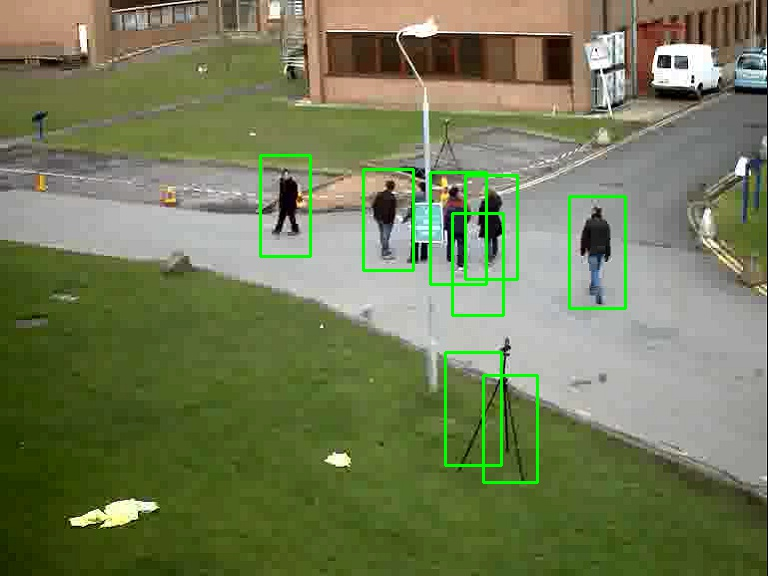
\includegraphics[width = \textwidth]{images/ImageDetector.jpg}
            \end{minipage}%
        }%
        \subfigure[BKGCutDetector]{\label{fig:sub:BKGCutDetector}
            \begin{minipage}[c]{0.5\textwidth}
            \centering
            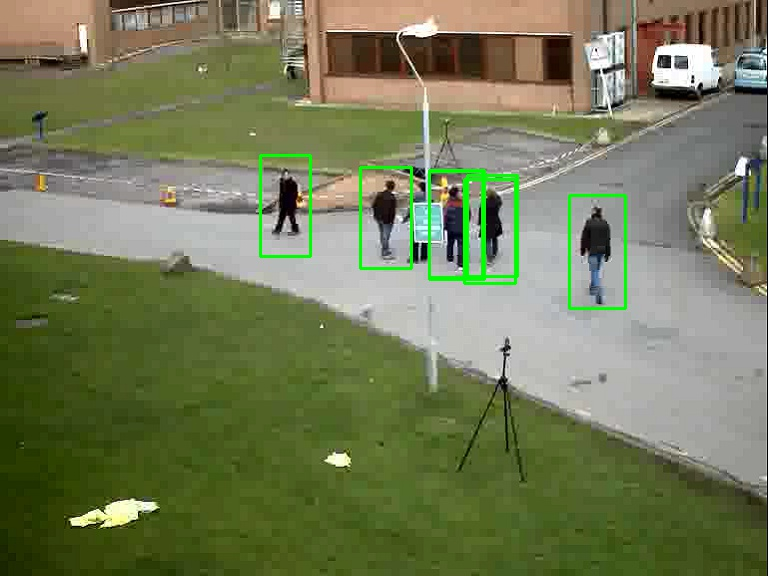
\includegraphics[width = \textwidth]{images/BKGCutDetector.jpg}
            \end{minipage}%
        }%
    \end{center}
    \caption{Detection Results}
    \label{fig:detector}
\end{figure}

\item Online Boosting

After the reconstruction, we start to work on the online boosting algorithm to track a single target. The main work is focus on Classifier part. We implement the following new classes.

\begin{itemize}

\item \lstinline{EstimatedGaussianDistribution}

Given a feature $f(\mathbf{x})$, the probability of $P(1|f(\mathbf{x}))$ and $P(-1|f(\mathbf{x}))$ is estimated as Gaussian distribution\cite{Grabner:2006:OBV:1153170.1153451}. This Gaussian distribution is estimated with Kalman filter\cite{Welch:1995:IKF:897831}. We use the following update equations for adaptive estimation from \cite{Grabner:2006:OBV:1153170.1153451}:

\begin{subequations}
\begin{align}
K_{t}&=\frac{P_{t-1}}{P_{t-1}+R}\\
\mathbf{\mu}_{t}&=K_{t}f(\mathbf{x})+(1-K_{t})\mathbf{\mu}_{t-1}\\
\mathbf{\sigma}_{t}^{2}&=K_{t}(f(\mathbf{x})-\mathbf{\mu}_{t})^{2}+(1-K_{t})\mathbf{\sigma}_{t-1}^{2}\\
P_{t}&=(1-K_{t})P_{t-1}
\end{align}
\end{subequations}

\item \lstinline{ClassifierThreshold}

It estimates the Gaussian distribution for both positive features $N(\mathbf{\mu_{+}}, \mathbf{\sigma_{+}})$ and negative features $N(\mathbf{\mu_{-}}, \mathbf{\sigma_{-}})$. Then it uses a simple distance threshold to a new feature to whether positive or negative: $h(\mathbf{x})$ for "hypothesis"

\begin{equation}
h(\mathbf{x})=\min_{+, -}(D(f(\mathbf{x}), \mu_{+}), D(f(\mathbf{x}), \mu_{-}))
\end{equation}

where $D(f(\mathbf{x}), \mu)$ is just the Euclidean distance in feature space.

\item \lstinline{WeakClassifierHaar}

It uses the Haar-like feature above and the \lstinline{ClassifierThreshold} to build a weak classifier. For classify, it uses \lstinline{HaarFeature} to extract the feature and sends it to \lstinline{ClassifierThreshold} to classify. For training, it uses the Kalman filter in \lstinline{EstimatedGaussianDistribution}.

\item \lstinline{ClassifierSelector}

Given a pool of weak classifiers, the \lstinline{ClassifierSelector} selects the best one with lowest error rate.

\begin{itemize}

\item Training

Each training feature $f(\mathbf{x})$ has an importance $\lambda$, and we use the idea from \cite{Oza01onlinebagging} to draw a random variable $k\sim Poisson(\lambda)$ and this feature is trained for $k$ times.

\item Selecting

For each weak classifier, we maintain two vaiables $\lambda_{correct}$ and $\lambda_{wrong}$:

\begin{subequations}
\begin{align}
\lambda_{correct}&=\sum_{i_{correct}}\lambda_{i}\\
\lambda_{wrong}&=\sum_{i_{wrong}}\lambda_{i}
\end{align}
\end{subequations}

And the error rate is estimated by:

\begin{equation}
err=\frac{\lambda_{wrong}}{\lambda_{correct}+\lambda_{wrong}}
\end{equation}

Then we choose the best weak classifier with lowest error rate.

\item Replacing

To improve the performance, each time we not only choose the best weak classifier but also replace the worst one with a randomly generated new weak classifier.

\end{itemize}

\item \lstinline{StrongClassifier}

The \lstinline{StrongClassifier} has $N$ \lstinline{ClassifierSelector}s, each with a voting weight $\alpha_i$. The final hypothesis is:

\begin{equation}
h^{strong}(\mathbf{x})=\mathrm{sign}(\sum_{i=1}^{N}\alpha_{i}\cdot h^{selector}_{i}(\mathbf{x}))
\end{equation} 

Suppose $err_i$ is the error rate of the $i^{th}$ selector, and then the voting weight is:

\begin{equation}
\alpha_i=\ln(\frac{1-err_i}{err_i})
\end{equation}

And the importance of this sample is updated with:

\begin{subequations}
\begin{align}
\lambda_{i+1}&=\lambda_i\cdot\sqrt{\frac{err_i}{1-err_i}}, &if~h^{selector}_{i}~correct\\
\lambda_{i+1}&=\lambda_i\cdot\sqrt{\frac{1-err_i}{err_i}}, &if~h^{selector}_{i}~wrong
\end{align}
\end{subequations}
\end{itemize}

\item Particle Filter

After we have the online boosting strong classifier. We try to combine it with particle filter.

\begin{itemize}

\item \lstinline{SingleSampler}

Given a target, it samples around it the positive and negative samples using Gaussian noise. Here is the samples: Figure~\ref{fig:singlesampler}, red for negative samples and blue for positive ones.

This is used in training the classifier.

\begin{figure}[htb]
    \begin{center}
        \subfigure[SingleSampler]{\label{fig:sub:singlesampler}
            \begin{minipage}[c]{0.5\textwidth}
            \centering
            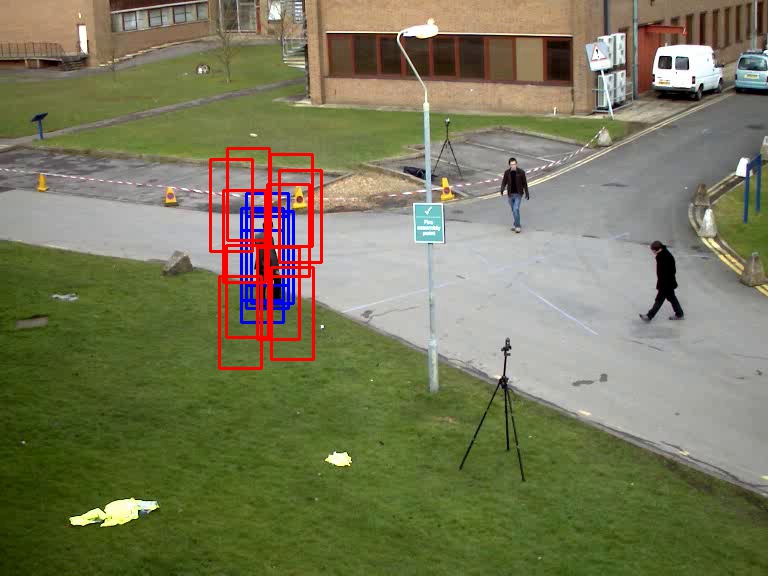
\includegraphics[width = \textwidth]{images/SingleSampler.jpg}
            \end{minipage}%
        }%
    \end{center}
    \caption{Detection Results}
    \label{fig:singlesampler}
\end{figure}

\item \lstinline{ParticleFilter}

This is a basic particle filter. The state space is just the position $[upper, left]$. The motion model is also very simple:

\begin{equation}
p_{t}=p_{t-1}+N(0, \sigma)
\end{equation}

where $N(0, \sigma)$ is a Gaussian random variable with variance proportional to the size of the target.

As for observation, it just use the scores given by strong classifier as the weight of the particles and resample it. We may improve the motion model later.

\item \lstinline{ParticleFilterTracker}

This class just combines everything together, use particle filter and strong classifier to track a target.

\end{itemize}

\item Result

With the following configuration we tested our single tracker on a small video clip. The result can be found \href{https://zerowong.github.io/PedestrainCounting/results/singleTrackerTestGray01.avi}{here}.

\begin{itemize}

\item The online boosting classifier is built with grayscale haar-like feature.
\item The particle filter just selects the best particle as the target and resamples around it.
\item 500 particles.
\item User initializes the target bounding box.

We can see that the classifier works quite good in Figure~\ref{fig:particlesConfidence}. After observation, the particles are drawn with their confidence. The brighter the particle is, the more confidence it has. Notice that the particle is at the upper-left corner of the target.

\begin{figure}[htb]
    \begin{center}
        \subfigure[]{\label{fig:sub:particlesConfidence}
            \begin{minipage}[c]{0.5\textwidth}
            \centering
            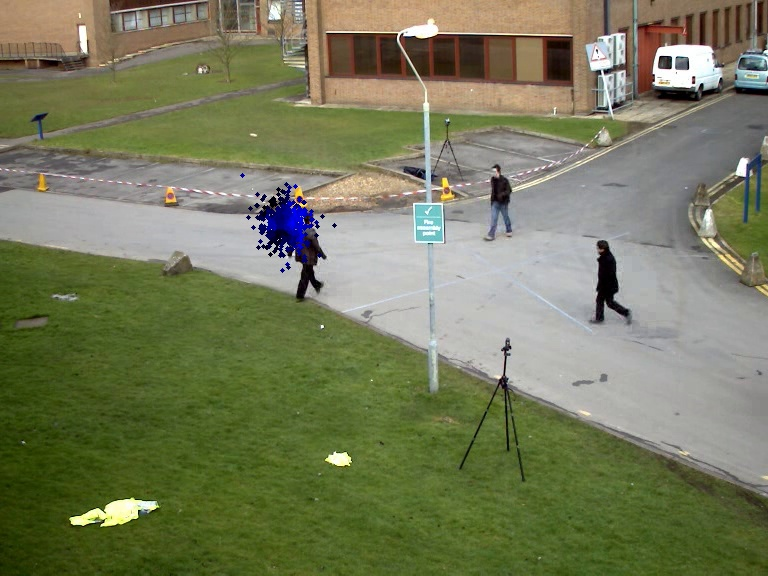
\includegraphics[width = \textwidth]{images/ParticlesConfidence.jpg}
            \end{minipage}%
        }%
    \end{center}
    \caption{Particles Confidence}
    \label{fig:particlesConfidence}
\end{figure}

\end{itemize}

\item RGI feature

From Figure~\ref{fig:singleTrackerGrayExchange} we can see that the current classifier can still not distinguish different pedestrains. We think this is due to the grayscale haar-like feature doesn't contain enough information. \cite{eth_biwi_00633} reports that with RGI (Red, Green, Intensity) histogram feature, 3 bins for each channel the results are quite good. 

Hence we implement \lstinline{RGIIntegralImage}, \lstinline{RGIFeature} and \lstinline{WeakClassifierRGI}. These classes use RGI feature to construct the weak classifier. The resulting video can be found \href{https://zerowong.github.io/PedestrainCounting/results/singleTrackerTestRGI01.avi}{here}. From this video and Figure~\ref{fig:singleTrackerRGIExchange} we can see that the classifier is more robustic and can handle some situation as two people crossing each other. However in Figure~\ref{fig:sub:singleRGI02} the classifier still goes for wrong pedestrain! Well they wear the same jeans I guess...

Well we need more code to solve this data association problem.

\begin{figure}[htb]
    \begin{center}
        \subfigure[Original target]{\label{fig:sub:singleGray01}
            \begin{minipage}[c]{0.5\textwidth}
            \centering
            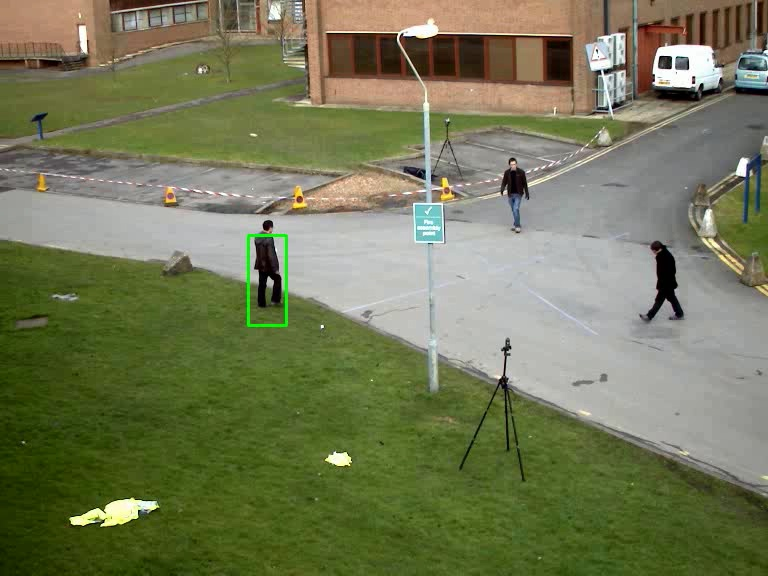
\includegraphics[width = \textwidth]{images/SingleTrackerGrayExchange01.jpg}
            \end{minipage}%
        }%
        \subfigure[Drift to another target]{\label{fig:sub:singleGray02}
            \begin{minipage}[c]{0.5\textwidth}
            \centering
            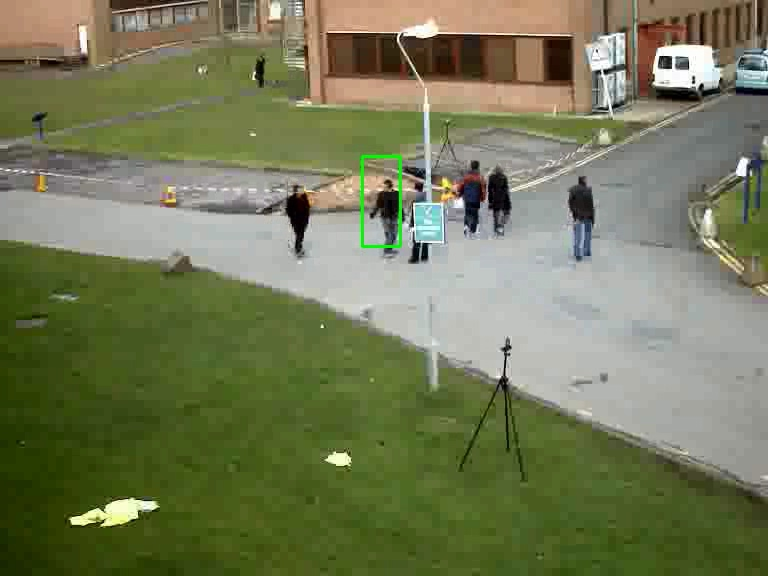
\includegraphics[width = \textwidth]{images/SingleTrackerGrayExchange02.jpg}
            \end{minipage}%
        }%
    \end{center}
    \caption{With grayscale haar-like feature, the tracker lost its target.(Black for original target)}
    \label{fig:singleTrackerGrayExchange}
\end{figure}

\begin{figure}[htb]
    \begin{center}
        \subfigure[Original target]{\label{fig:sub:singleRGI01}
            \begin{minipage}[c]{0.5\textwidth}
            \centering
            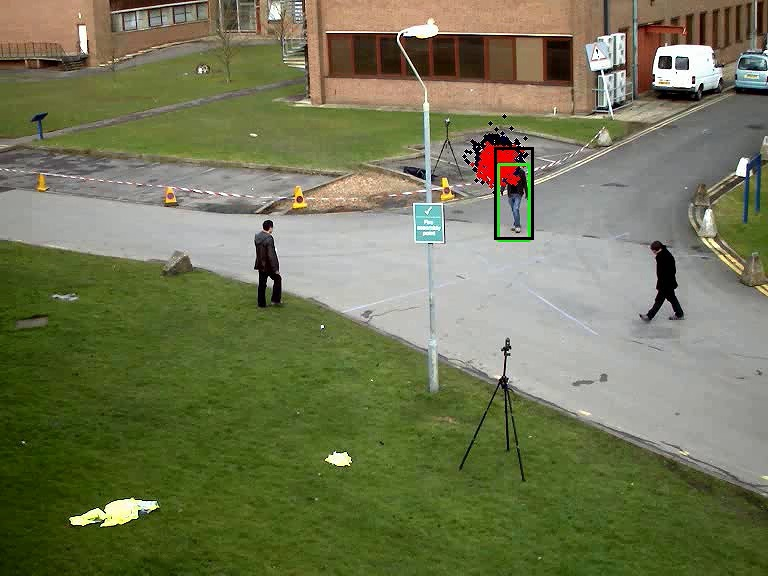
\includegraphics[width = \textwidth]{images/SingleTrackerRGIExchange01.jpg}
            \end{minipage}%
        }%
        \subfigure[Drift to another target]{\label{fig:sub:singleRGI02}
            \begin{minipage}[c]{0.5\textwidth}
            \centering
            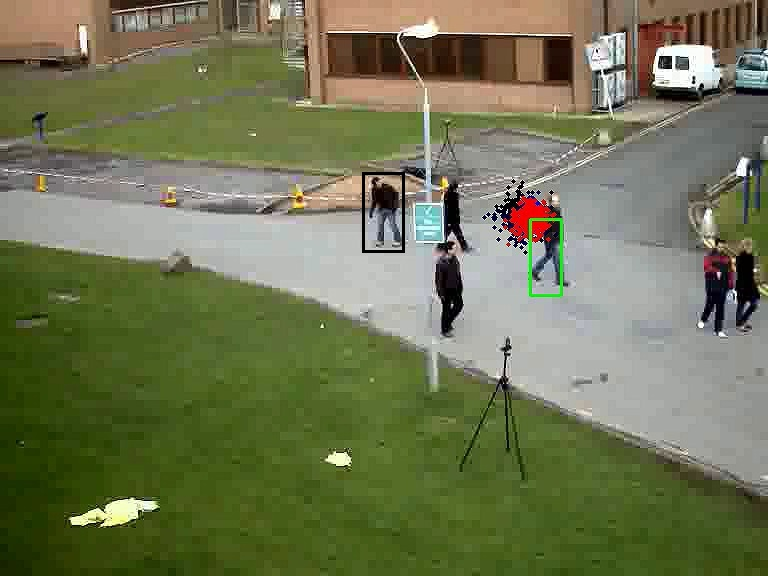
\includegraphics[width = \textwidth]{images/SingleTrackerRGIExchange02.jpg}
            \end{minipage}%
        }%
    \end{center}
    \caption{With RGI feature, the tracker is more robustic, but still lost its target finally. (Black for original target)}
    \label{fig:singleTrackerRGIExchange}
\end{figure}

\end{itemize}

\item \textbf{Further Plan}

\begin{itemize}

\item Mean-shift to find the target

Now the particle filter just selects the best particle as the target, and resamples arount it. However this loses almost every advantage of particle filter. So our next plan is to use mean-shift to find the target from all these particles.

\item Multi-target Tracker

This is our final object. The main problem is data association. We are not sure we will be able to finish this. But we will see.

\end{itemize}


\item \textbf{Experiment}

All the experiment is executed on Dell Inspiron 14R SE with the following configuration.
All the experiment result can be found \href{https://zerowong.github.io/PedestrainCounting/results/}{here}.

\begin{itemize}

\item Intel Core i7-3612QM 2.10GHz
\item 8.00GB RAM
\item System: Windows 8.1 x64
\item OpenCV: 3.00

\end{itemize}

For video we have three clips: \href{https://zerowong.github.io/PedestrainCounting/results/test/1.avi}{1.avi}, \href{https://zerowong.github.io/PedestrainCounting/results/test/2.avi}{2.avi}, \href{https://zerowong.github.io/PedestrainCounting/results/test/3.avi}{3.avi}.

For single image detection we only use \href{https://zerowong.github.io/PedestrainCounting/results/test/test.jpg}{test.jpg}, which is from \href{https://zerowong.github.io/PedestrainCounting/results/test/1.avi}{1.avi}.

The original baseline program is tested with all default settings.

\begin{itemize}

\item HoG Detector.

We first use the simple HoG detector to detect a single picture.
\begin{center}
\begin{tabular}{l | c | c | r}
\hline
                & Time  & Accuracy  & False Positive \\
Original        & 3.43s & 5 / 6     & 3              \\
Reconstructed   & 3.20s & 5 / 6     & 2              \\
\hline
\end{tabular}
\end{center}

\item Background Cut Detector.

We use the simple Background cut detector to detect pedestrain in a single picture.

\begin{center}
\begin{tabular}{l | c | c | r}
\hline
                & Time  & Accuracy  & False Positive \\
Original        & 1.76s & 6 / 6     & 0              \\
Reconstructed   & 1.27s & 5 / 6     & 0              \\
\hline
\end{tabular}
\end{center}

\item HoG Detector for Video.

We use the simple HoG detector to detect pedestrain in a video.

\begin{center}
\begin{tabular}{l | c | c | r}
\hline
                & Time  & Accuracy  & False Positive \\
Original        & 1051s  &           &                \\
Reconstructed   & 900s &           &                \\
\hline
\end{tabular}
\end{center}

\item Background Cut Detector for Video.

We use the simple Background Cut detector to detect pedestrain in a video.

\begin{center}
\begin{tabular}{l | c | c | r}
\hline
                & Time  & Accuracy  & False Positive \\
Original        & 207.36s  &           &                \\
Reconstructed   & 159.14s  &           &                \\
\hline
\end{tabular}
\end{center}

\end{itemize}

\end{enumerate}

\clearpage
\bibliographystyle{plain}
\bibliography{Ref}

\end{document}
